\begin{figure}
    \centering
    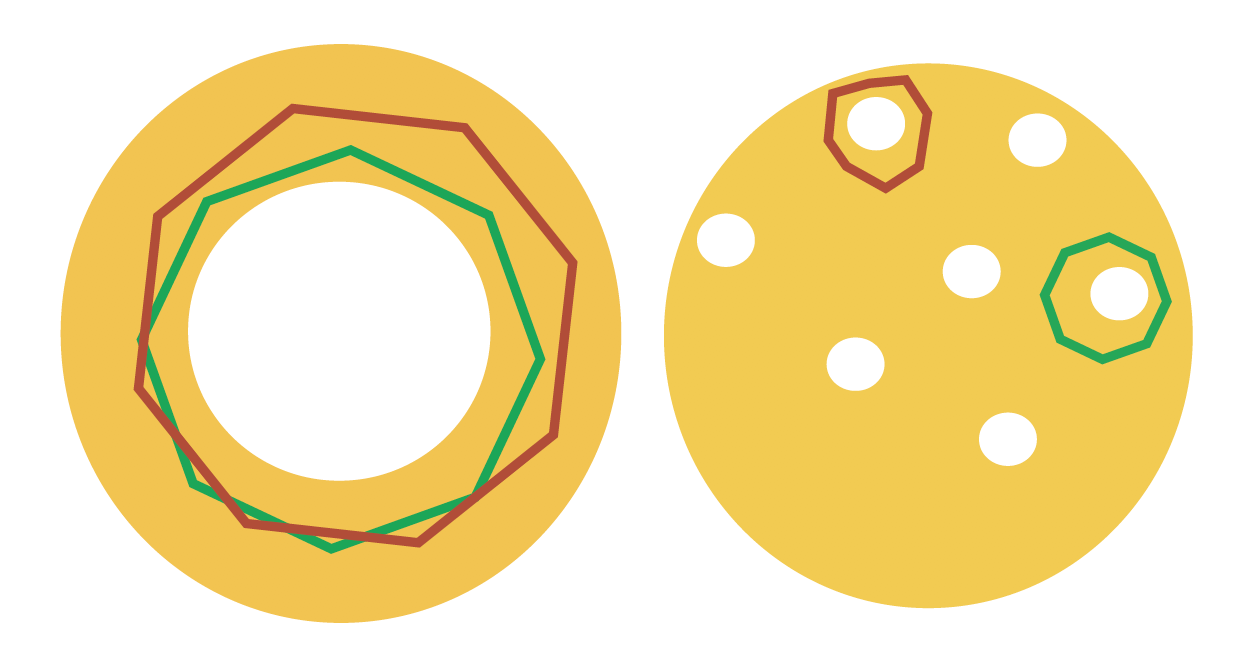
\includegraphics[width=0.8\textwidth]{figures/generatorExample.png}
    \caption{Two disks (yellow) --- which we regard as 2-dimensional simplicial complexes, though the explicit decomposition into simplices is not shown --- with different numbers of holes (white) and cycle representatives (red or green) from \cite{Carlsson2009TopologyAD}. The disk on the left has a single 2-dimensional  ``hole'' ($\beta_1 = 1$), and the two loops around it are cycle representatives for the same homology class. Similarly, the disk on the right has seven ``holes'' ($\beta_1 = 7$) and the two loops shown are cycle representatives for different homology classes.
    }
    \label{fig:generatorExamples}
\end{figure}
